\section{Leak-Free Benchmarks and Evaluation Protocol}
\label{sec:benchmarks}

\subsection{Splits}
\textbf{WTBD-group.} The 1{,}065 WTBD images are split by scene into 745/159/161 images, the official sizes. The split holds 1{,}109/240/235 boxes and 224/60/58 scene groups. It was audited until no held-out image matched the training set under DINOv2 and ORB verification. The 25\% and 50\% label fractions are nested subsets of the training scenes.

\textbf{WTBlade-group.} We start from 10{,}527 WTBlade-Defect images, leaving out the 133 that match WTBD so that the two benchmarks share nothing. From them we form 841 groups out of 2{,}791 source frames, verified pairs and DINOv2 neighbours. A class-stratified 70/15/15 split over groups converged with no held-out-to-train match after 11 rounds of the audit. We keep one image per source frame, giving 2{,}136/323/332 frames, 5{,}237/729/748 boxes and 177 test scenes, with all seven classes in every split.

\textbf{A residual leak in our own splits.} While building a later pool, we added the pixel test to our audit and ran it on these splits. It found copies that DINOv2 and ORB had missed: 6 of 161 test and 6 of 159 validation images on WTBD-group, and 1 of 332 and 1 of 323 on WTBlade-group (Fig.~\ref{fig:residual}). All six WTBD-group test pairs are real copies by eye, re-exposed, darkened, tinted or rotated. We rescored 116 cached WTBD-group runs without those images. This changes \mcoco by $-0.62$ on average (range $-1.09$ to $+0.33$) and \mfifty by $-0.70$; 20 WTBlade-group runs change by $\pm0.03$. Our leak-free numbers are therefore inflated by under a point. We kept the splits unchanged, so that every comparison stays like for like, and we report every pre-registered decision both ways. None changes. A leak-free split needs the pixel test next to scene grouping, and ``audited'' is only as good as the audit.

\begin{figure}[!t]
\centering
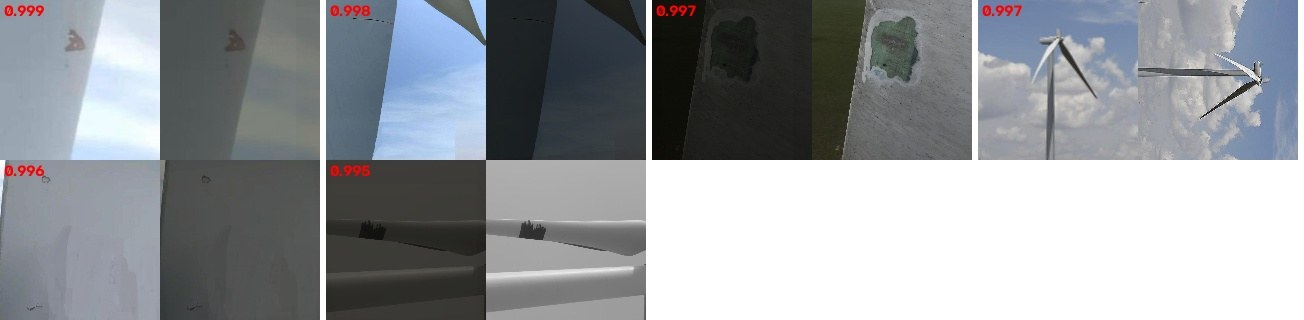
\includegraphics[width=\linewidth]{fig28_residual_twins}
\caption{The residual leak in our WTBD-group test set: each pair is a test image and its pixel twin in train, with the correlation. Photometric copies defeat DINOv2 + ORB grouping.}
\label{fig:residual}
\end{figure}

\subsection{Selection and Reporting}
Model selection uses validation only, and results are reported on test, scored once. Wind Surface has no separate test split, so we carve a seeded 10\% of its training set for validation (2{,}570/286/714). Unless stated otherwise, ``points'' are percentage points of AP.

\subsection{Evaluator}
We use a 101-point COCO-style evaluator~\cite{coco,pascal} (\texttt{tools/bootstrap\_ci.py}). On identical predictions it agrees with Ultralytics' \texttt{ap\_per\_class}~\cite{ultralytics} within 0.4 points on every run and subset, so the gaps to published figures are not an artefact of the metric. Ultralytics' \texttt{val} reports differ by 1--2.5 points from cached predictions, because of its rectangular-batch inference path. Tables state which evaluator they use.

\subsection{Scene Bootstrap}
Test images of one scene are correlated, so intervals that resample images are too narrow~\cite{fieldwelsh}. Let $\mathcal{G}=\{g_1,\dots,g_S\}$ be the test scene groups. A replicate draws $S$ groups with replacement, $\mathcal{G}^{*b}$, and recomputes the metric on the union of their images. For a paired comparison between models $A$ and $B$ that both predicted every test image,
\begin{equation}
\Delta^{*b} = M_A\!\left(\textstyle\bigcup_{g\in\mathcal{G}^{*b}} g\right) - M_B\!\left(\textstyle\bigcup_{g\in\mathcal{G}^{*b}} g\right),
\label{eq:bootstrap}
\end{equation}
with the same draw used for both models. We report the 2.5 and 97.5 percentiles of $\{\Delta^{*b}\}_{b=1}^{2000}$ and $P(\Delta>0)=\frac{1}{B}\sum_b\mathbb{1}[\Delta^{*b}>0]$~\cite{efron}. With two training seeds, $\Delta$ is the mean over seeds within each replicate. With two datasets, the dataset mean is taken within each replicate, with independent draws per dataset. The official splits have no scene groups, so their intervals resample images and are therefore narrower than they should be.

\subsection{Three Box Scores}
\textit{Standard} AP uses one-to-one matching at IoU~$\geq 0.5$ (\apfifty) or averaged over IoU 0.50:0.95 (\mcoco). \textit{Tolerant} AP lets one prediction match several same-class labels whose union it fits, and ignores fragments of an already found defect. \textit{Region} AP is the pixel-level precision and recall of the union of predicted boxes against the union of labels, on a 4-px grid. For a class $c$ at confidence threshold $\theta$,
\begin{equation}
P_c(\theta)=\frac{|\,\cup\hat{B}_c(\theta)\cap\cup B_c\,|}{|\,\cup\hat{B}_c(\theta)\,|},\quad
R_c(\theta)=\frac{|\,\cup\hat{B}_c(\theta)\cap\cup B_c\,|}{|\,\cup B_c\,|},
\label{eq:region}
\end{equation}
and region AP is the area under $(R_c,P_c)$. It does not depend on how a defect is cut into boxes. A trivial detector that boxes the whole image scores 14--24 region AP on our benchmarks, so raw region AP must be read against that floor.

\subsection{Pre-Registration}
From late October onwards, hypotheses were written down with their pass bars before any run or computation, and committed to the repository~\cite{prereg,repo}. A typical primary claim reads: ``the paired difference is $>0$ on each dataset, and the dataset mean has $P(\Delta>0)\geq0.95$''. After a bad result we allow one scope check, on whether any part is usable, and then discard the hypothesis without rescue runs. Post hoc analyses are labelled as such throughout.
